% Blocks: two cohorts sit in one B for one of two reasons, and which one it is
% decides how the block is resampled.
%
%   compile:  pdflatex blocks.tex
%
\documentclass[border=10pt]{standalone}
\usepackage{lmodern}
\usepackage{amsmath}
\usepackage{amssymb}
\usepackage{tikz}
\usetikzlibrary{arrows.meta,positioning,calc}
% Shared palette for the population-model figures.
%   ink      body / structure
%   popcol   the patient cloud and anything predicted from it
%   mechcol  the simulator and species-level quantities
%   msrcol   the measurement map (readout-level: gamma, kappa)
%   datacol  reported rows
\definecolor{ink}{HTML}{3A3A3A}
\definecolor{popcol}{HTML}{3B4AA6}
\definecolor{mechcol}{HTML}{2E7D5B}
\definecolor{msrcol}{HTML}{EB811B}
\definecolor{datacol}{HTML}{8C3B4A}

\newcommand{\Bset}{\mathcal{B}}

\begin{document}
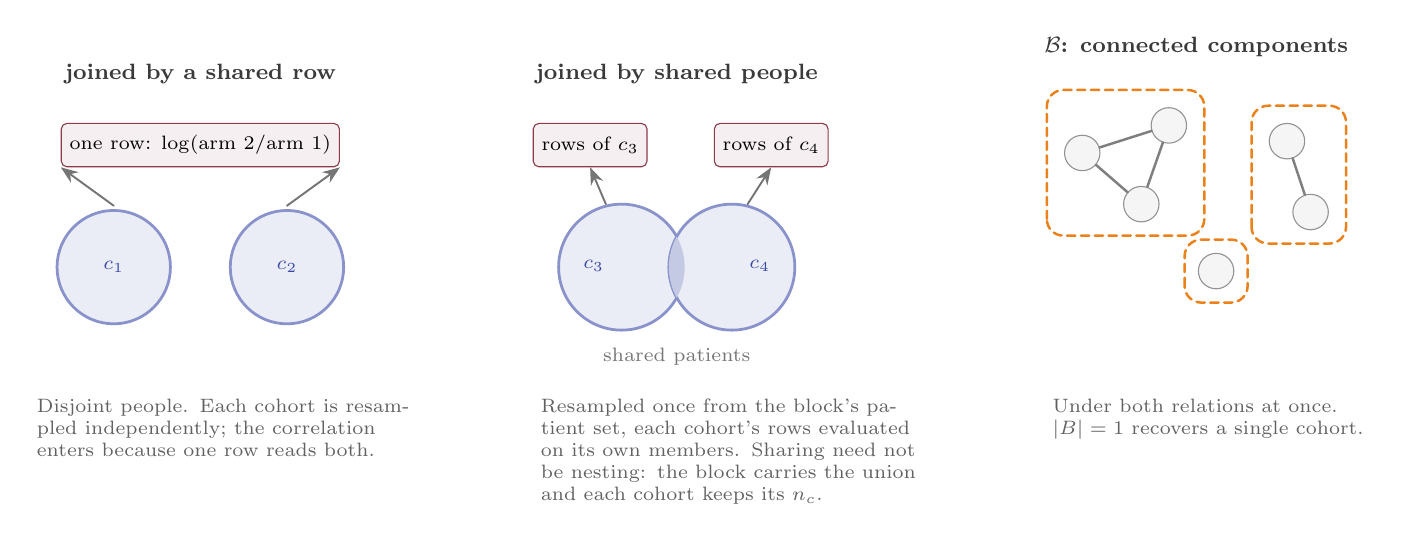
\begin{tikzpicture}[
  font=\sffamily, >=Stealth, line cap=round, line join=round,
  row/.style={draw=datacol, fill=datacol!8, rounded corners=2pt,
              minimum height=5.5mm, inner sep=3pt, font=\scriptsize},
  ttl/.style={font=\footnotesize\bfseries, anchor=south},
  figcap/.style={font=\scriptsize, text=ink!80, align=left, anchor=north west},
  fl/.style={-{Stealth[length=2.2mm]}, ink!70, line width=0.7pt}]

% ================================================ (i) joined by a shared row
\begin{scope}[shift={(0,0)}]
  \draw[popcol!60, fill=popcol!10, line width=1pt] (0.9,0) circle (0.72);
  \draw[popcol!60, fill=popcol!10, line width=1pt] (3.1,0) circle (0.72);
  \node[popcol, font=\scriptsize] at (0.9,0) {$c_1$};
  \node[popcol, font=\scriptsize] at (3.1,0) {$c_2$};
  \node[row] (r) at (2.0,1.55) {one row: $\log(\text{arm }2/\text{arm }1)$};
  \draw[fl] (0.9,0.78) -- (r.south west);
  \draw[fl] (3.1,0.78) -- (r.south east);
  \node[ttl, ink] at (2.0,2.20) {joined by a shared row};
\end{scope}
\node[figcap, text width=48mm] at (-0.2,-1.55)
  {Disjoint people. Each cohort is resampled independently; the correlation
   enters because one row reads both.};

% ================================================ (ii) joined by shared people
\begin{scope}[shift={(6.4,0)}]
  \draw[popcol!60, fill=popcol!10, line width=1pt] (0.95,0) circle (0.80);
  \draw[popcol!60, fill=popcol!10, line width=1pt] (2.35,0) circle (0.80);
  \begin{scope}
    \clip (0.95,0) circle (0.80);
    \fill[popcol!30] (2.35,0) circle (0.80);
  \end{scope}
  \node[popcol, font=\scriptsize, anchor=east] at (0.85,0.02) {$c_3$};
  \node[popcol, font=\scriptsize, anchor=west] at (2.45,0.02) {$c_4$};
  \node[ink!70, font=\scriptsize, anchor=north] at (1.65,-0.90) {shared patients};
  \node[row] (r3) at (0.55,1.55) {rows of $c_3$};
  \node[row] (r4) at (2.85,1.55) {rows of $c_4$};
  \draw[fl] (0.75,0.80) -- (r3.south);
  \draw[fl] (2.55,0.80) -- (r4.south);
  \node[ttl, ink] at (1.65,2.20) {joined by shared people};
\end{scope}
\node[figcap, text width=48mm] at (6.2,-1.55)
  {Resampled once from the block's patient set, each cohort's rows evaluated on
   its own members. Sharing need not be nesting: the block carries the union and
   each cohort keeps its $n_c$.};

% ================================================ (iii) the partition
\begin{scope}[shift={(13.2,0.35)}]
  \foreach \n/\x/\y in {a/0/1.1, b/1.1/1.45, c/0.75/0.45, d/2.6/1.25, e/2.9/0.35, f/1.7/-0.40}
    \node[circle, draw=ink!55, fill=ink!5, minimum size=4.5mm, inner sep=0pt,
          font=\tiny] (\n) at (\x,\y) {};
  \draw[ink!65, line width=0.9pt] (a) -- (b);
  \draw[ink!65, line width=0.9pt] (a) -- (c);
  \draw[ink!65, line width=0.9pt] (b) -- (c);
  \draw[ink!65, line width=0.9pt] (d) -- (e);
  \draw[msrcol, rounded corners=6pt, line width=0.9pt, densely dashed]
    (-0.45,0.05) rectangle (1.55,1.9);
  \draw[msrcol, rounded corners=6pt, line width=0.9pt, densely dashed]
    (2.15,-0.05) rectangle (3.35,1.7);
  \draw[msrcol, rounded corners=6pt, line width=0.9pt, densely dashed]
    (1.30,-0.80) rectangle (2.10,0.00);
  \node[ttl, ink] at (1.45,2.20) {$\Bset$: connected components};
\end{scope}
\node[figcap, text width=40mm] at (12.7,-1.55)
  {Under both relations at once. $|B|=1$ recovers a single cohort.};

\end{tikzpicture}
\end{document}
